\section{深層類神經網路}

\subsection{簡介}
深層類神經網路以及深層學習,是機器學習中相當重要的一個分支,曾於 1980 年代蓬勃發展,但因所需計算代價過於巨大,在當時電腦沒有足夠的能力來處理大型神經網路所需要很長的計算時間,直到電腦具有更強的計算能力之前,神經網路的研究進展緩慢。深層學習的概念由辛氏(Geoffrey Hinton)於 2006 重新推出,並使用一種新型的訓練方法,能夠有效提升訓練的速度;再加上硬體圖形處理器( Graphics Processing Unit, GPU)的高度發展,大幅提高了數值和矩陣運算的速度,種種原因使得深層類神經網路重新成為機器學習領域,甚至在 2015 年, Google 為了深度學習分別在軟硬體推出了 TensorFlow \cite{tensorflow2015-whitepaper} 以及 TPU(Tensor Processing Unit) \cite{jouppi2017datacenter} 來加速這領域的發展。

\subsection{運作原理}
深層類神經網路發想於人類中樞神經系統,在深層類神經網路中,簡單的人工節點,稱作神經元(Neuron),連線在一起形成一個類似生物神經網路的網狀結構。根據此仿生的觀察,便產生一種數學模型,將神經元規劃為層狀結構,把輸入特徵(Input Feature)通過一層一層的感知器(Perceptron)或稱隱藏層(Hidden Layer),傳遞到最後一層輸出層(Output Layer),進行多類別分類(Multiclass Classification),而多個感知器傳接而成,又稱為多層感知器(Multi-layer Perceptron, MLP)。每一層根據所在位置可分為三類:
\begin{itemize}
    \item 輸入層:眾多神經元接受大量非線形輸入訊息,輸入的訊息稱為輸入向量 $\bold{x} = [x_1,x_2, ... , x_M]$ 。
    \item 輸出層:訊息在神經元鏈接中傳輸、分析、權衡,形成輸出結果。輸出的訊息稱為輸出向量 $\bold{y} = [y_1,y_2,...y_n]$ ,與標記種類(Class)一樣多
    \item 隱藏層:可有一層以上。是輸入層和輸出層之間眾多神經元和鏈接組成。
\end{itemize}
每個感知器都包含了一組加權係數、偏移量(Bias),以及一個非線性的活化函數(Activation Function)。此數學模型可表示成:
\begin{figure}[h]
    \centering
    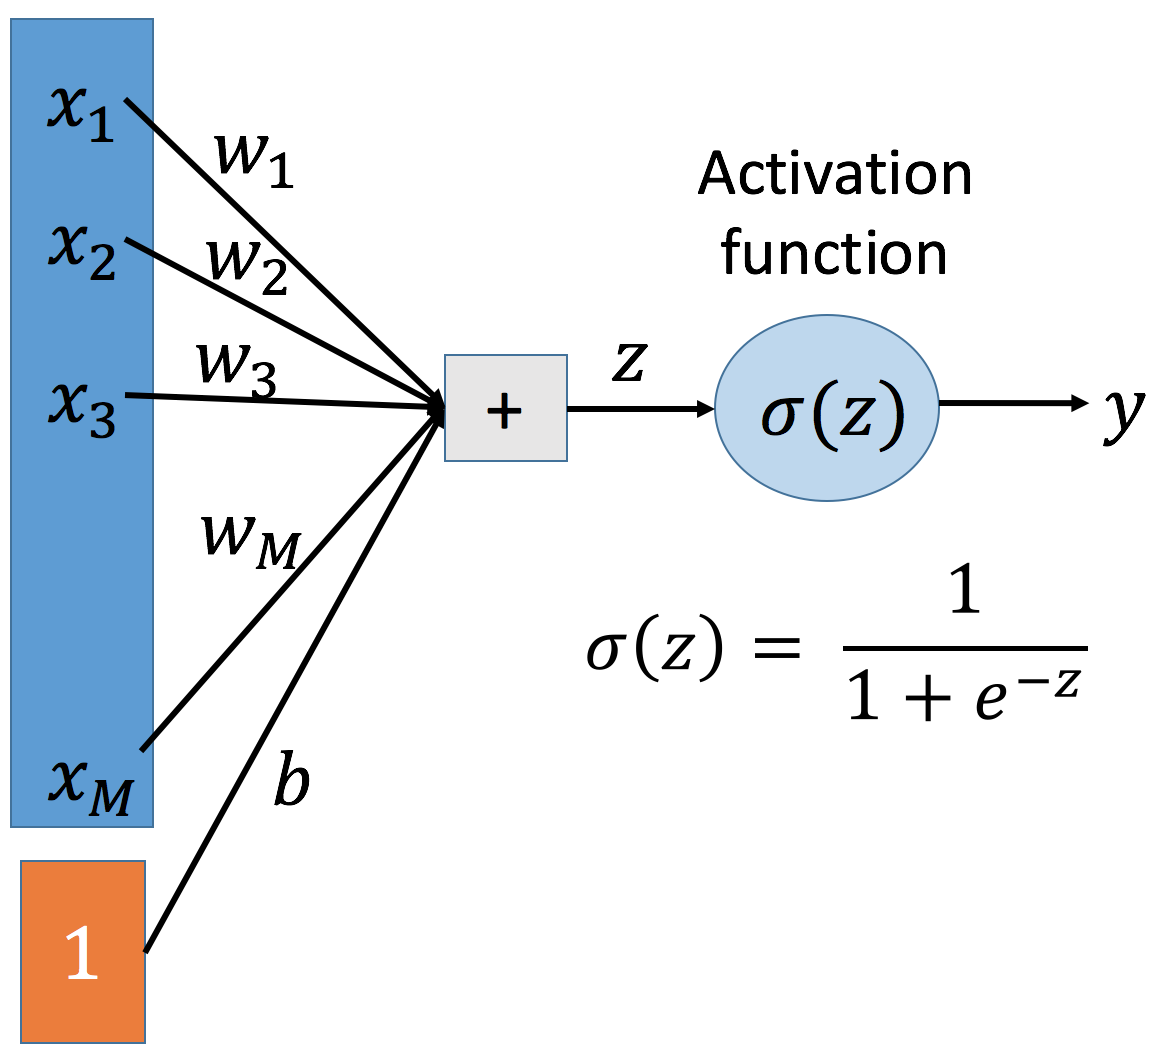
\includegraphics[scale=0.4]{images/chap2_perceptron.png}
    \caption{感知器示意圖}
\end{figure}
\begin{equation}
    y_i = \sigma{(\sum_{i=1}^M w_{ij}x_i+b_j)} ,  j= 1,...,N
\end{equation}
其中 $\sigma$ 為活化函數,$w_{ij}$ 是第 $j$ 個感知器中,對應到第 $i$ 個輸入 $x_i$ 的加權係數,$b_j$ 是第 $j$ 個感知器的偏移量。

在上面的式子中, $\sigma$ 括號內代表輸入向量都會經由仿射變換(Affine Transform),我們可以將此轉換視為從 $M$ 維的實數空間映射至 $N$ 維的實數空間函數 $f:R^M \rightarrow R^N$ ,也就是一個線性矩陣轉換,因此需要使用活化函數提升複雜度。

一般來說,只要是非線性函數(Nonlinear Function)都可以當成活化函數,而常見的活化函數有如S型函數(Sigmoid)和整流線型單元(Rectified Linear Unit, ReLU),分別為:
%TODO Add Sigmoid Figure
\begin{equation}
    sigmoid(x) = \frac{1}{1 + e^{-x}}
\end{equation}
\begin{equation}
    ReLU(x) = max(0,x)
\end{equation}
另外如果我們想要訓練一個分類器(Classifer),通常在最後一層的非線性函數會選擇軟性最大化(Softmax)作為活化函數。
\begin{equation}
    P(y = i|x)= softmax(x)_{i} = \frac{e^{x_i}}{\sum_j^N e^{x_j}}
\end{equation}

\subsection{訓練方法}
深層類神經網路的訓練方式,需要借助損失函數(Loss Function),來模擬類神經網路與理想函數的量化距離:
\begin{equation}
    \theta^{\ast} = \arg\min_{\theta}{C(x,y;\theta)}
\end{equation}
其中 $\theta$ 是整個模型所需要的參數, $\theta^{\ast}$ 代表模型的最佳解(Optimal Solution),能夠使 $C(.)$ 最小化。

常見的損失函數有以下,例如均方差(Mean Squared Error)以及交叉熵(Cross Entropy, CE):
\begin{equation}
    C_{MSE}(x,y;\theta) = \frac{1}{N}\sum||f(x;\theta) - y||_{2}
\end{equation}
\begin{equation}
    C_{CE}(x,y;\theta) = -\sum_i y_i\log f(x;\theta)_i
\end{equation}
其中 $f(x;\theta)$ 為模型的輸出。 $C_{MSE}$ 是均方差的損失函數,單純將 $f(x;\theta)$ 和正確答案 $y$ 之間的歐式距離(Euclidean distance)的平均當損失函數,通常用來處理回歸(Regression)問題。 $C_{CE}(.)$ 則是交叉熵的損失函數。

當我們設計好模型以後,下一個問題便是要選擇一個模型的最佳解 $\theta^{\ast}$ ,以便得到最小的損失。由於參數介於實數之間,我們不可能使用暴力解窮舉所有可能來找出最佳解。通常我們所採取的是反向傳播演算法(Backpropagation Algorithm)來訓練深層類神經網路,反向傳播演算法是基於微分連鎖率(Chain Rule)的特性,搭配著梯度下降(Gradient Descent),也就給定一組參數 $\theta$ ,損失函數沿著該參數的梯度方向更新,可表示成:
\begin{equation}
    \theta_{k+1} \leftarrow \theta_k - \eta\Delta\theta_k
\end{equation}
\begin{equation}
    \Delta\theta_k = \frac{\partial C}{\partial\theta}\biggr|_{\theta = \theta_k}
\end{equation}
$k$ 為迭代(Iteration)的次數, $\eta$ 為學習率(Learning Rate),通常是一個相對小的數字,約在 0.1 到 0.001 不等,一般來說,要找到好的學習率是不容易的。大的學習率優點就是能讓學習速度變快,但相對來講可能會讓較難找到最佳解,可能使更新的路徑如同之字形(Zig-zag)般移動,甚至使損失函數越來越大;而過小的學習率會導致學習時間太久,迭代次數過多,所以通常會在一開始會挑一個較大的學習率,當損失函數不再下降,則會讓學習率衰減,以避免更新路徑如同之字形般移動,亦能更靠近最佳解。

而梯度下降因為是根據當前的參數去更新,其範圍僅侷限在前一次的參數位置的周圍,因此只有可能收斂在此參數空間的局部最小值(Local Minimum),而不一定是全域最小值(Global Minimum),無法保證能獲得最佳解。
%TODO? Adam/Momentum

\subsection{丟棄演算法}
由於深層類神經網路有很好的學習性,因而陷入了過度貼合(Overfitting)的狀況,即在訓練集裡的表現越來越好,但卻在測試集的表現越來越差,強記所有的訓練集的資料,並沒有學習到資料的特性。故我們需要一些方式來避免過度貼合,常見的有使用正規化(Regularization),可以降低模型的複雜度,但卻不會降低模型的強度,方法是在損失函數上額外添加控制參數大小的控制子,方式有稀疏正規化(sparsity regularization)和權重正規化/參數衰減正規化(L2/weight-decay regularization)兩種。
\begin{equation}
    C'(\theta) = C(\theta) + \frac{\lambda}{n}\Arrowvert\theta\Arrowvert
\end{equation}
\begin{equation}
    C'(\theta) = C(\theta) + \lambda\frac{1}{2}\Arrowvert\theta\Arrowvert^2
\end{equation}

\begin{figure}[t]
    \centering
    \subfloat[][標準類神經網路]{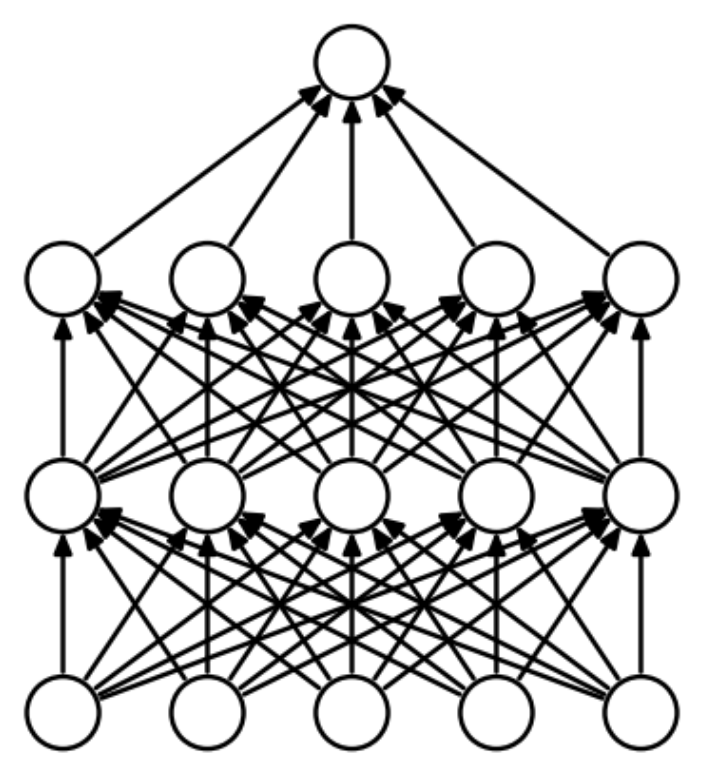
\includegraphics[scale=0.5]{images/chap2_stdNN.png} }
    \subfloat[][隨機丟棄部分神經元]{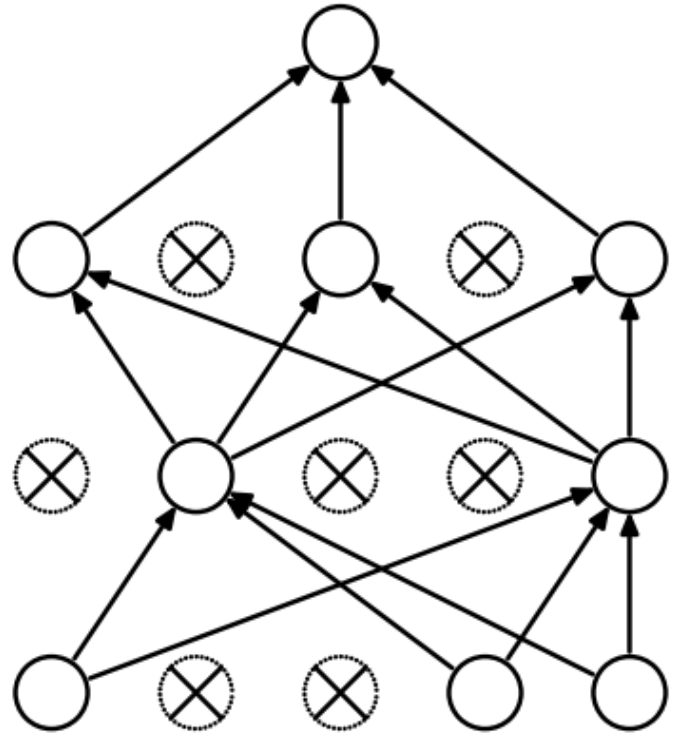
\includegraphics[scale=0.5]{images/chap2_dropout.png}}
    \caption{丟棄演算法示意圖\cite{srivastava2014dropout} }\label{fig:chap2_dropout} 
\end{figure}
另一種方法是對類神經網路而言,辛氏(Hinton)提出丟棄演算法(Dropout)~\cite{srivastava2014dropout} :即在訓練時,每個迭代保留 $p\%$ 的神經元,另外 $(1-p)\%$ 的神經元直接關閉,無法活化,使得輸出值為 0 ,如圖 \ref{fig:chap2_dropout} 。概念可以想成是希望每個神經元能自己學到參數,而不靠其他神經元,因而強迫神經元能學到更概括的能力。而當在訓練時丟棄 $(1-p)\%$ 的神經元,在測試則是使用所有的神經元,因此所有的參數需要乘上 $p\%$ 的權重來平衡,如圖 \ref{fig:chap2_drop_w}

\begin{figure}[h]
    \centering
    \subfloat[][訓練時]{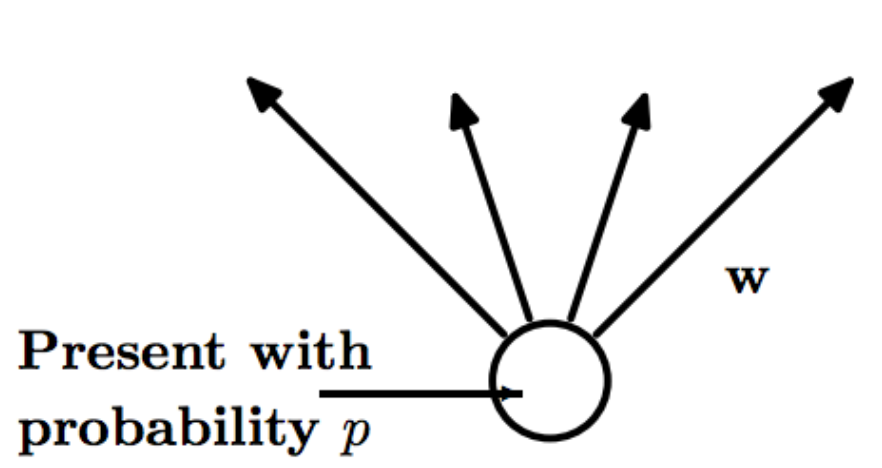
\includegraphics[scale=0.3]{images/chap2_drop_train.png}}
    \subfloat[][測試時]{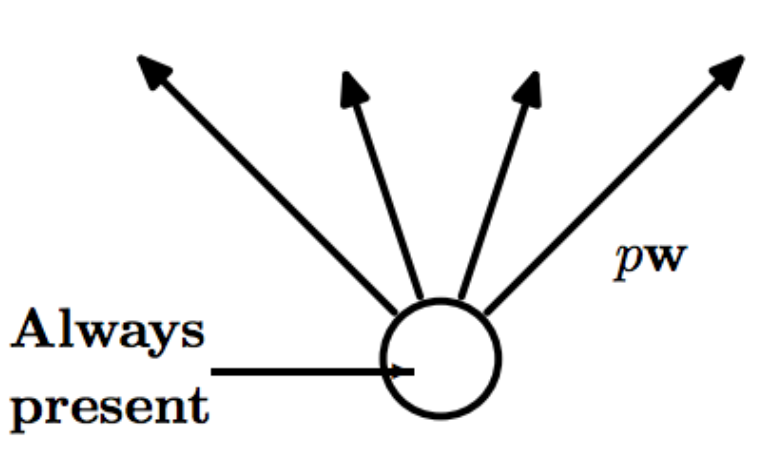
\includegraphics[scale=0.3]{images/chap2_drop_test.png}}
    \caption{丟棄演算法權重變化\cite{srivastava2014dropout}}\label{fig:chap2_drop_w}
\end{figure}

丟棄演算法也可以視為多個神經網路的隨機整合(Random Ensemble)。整合模型(Ensemble Model)在機器學習(Machine Learning)領域已經被證明是非常強大的模型,藉由多個模型的多樣性(Diversity)來提升模型的強度。在丟棄演算法中,每個迭代有不同的丟棄情況,就有不同架構的模型,這種隨機性造成了多樣性,才能使得模型不容易過度貼合。

\section{遞迴式神經網路(Recurrent Neural Network, RNN)}
\begin{figure}[b]
    \centering
    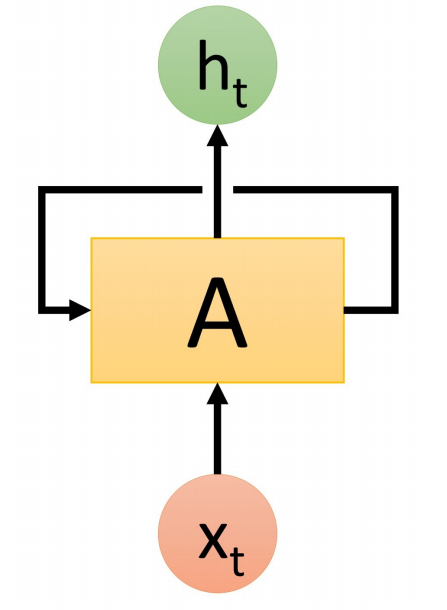
\includegraphics[scale=0.25]{images/chap2_rnn.png}
    \caption{遞迴式神經網路示意圖\cite{shen2016} }\label{fig:chap2_rnn}
\end{figure}
\subsection{簡介}
雖然深層類神經網路擁有很好的分類能力,但是當輸入資料呈現序列狀(Sequential),且有上下文關係(Context Dependency)時,如語音辨識(Speech Recongnition)、自然語言理解(Nature Language Understanding),這時候深層類神經網路就無法妥善處理。因此這時候需要記憶細胞(Memory Cell)來幫助,即是遞迴式類神經網路,圖 ~\ref{fig:chap2_rnn} 為其架構。不同於深層類神經網路,它是帶有循環的神經網路。在圖 ~\ref{fig:chap2_rnn} 中, $A$ 代表神經網路的主體, $x_t$ 代表在時間點 t 時的輸入, $h_t$ 代表在時間點 t 時的網路輸出,這種循環結構能使資訊從前面傳遞到後面,能夠允許資訊保留一段時間。我們將迴圈展開後,不難發現其可根據輸入資料的序列關係展開成一鏈狀結構,如圖 ~\ref{fig:chap2_unrollrnn} 所示,因此我們可以將遞迴神經網路想像成是有多層相同的神經網路,每一層都會將資訊傳遞給下一層。

\begin{figure}[h]
    \centering
    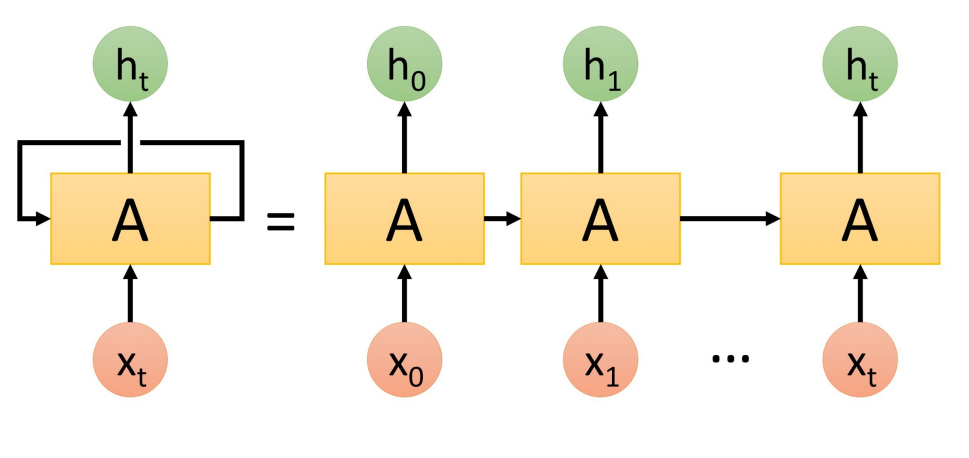
\includegraphics[scale=0.3]{images/chap2_unrollrnn.png}
    \caption{遞迴式神經網路展開示意圖\cite{shen2016} }\label{fig:chap2_unrollrnn}
\end{figure}

%\subsection{沿時間反向傳播演算法(Backpropagation through Time, BPTT)}
%訓練遞迴類神經網路的方法稱作沿時間反向傳播演算法 ,%TODO?
\subsection{長短期記憶神經網絡(Long Short-term Memory Network)}
雖然遞迴類神經網路的設計看起來能有效地處理序列狀的問題,但實作後發現,遞迴類神經網可能會有梯度爆炸或者梯度消失的問題,並無法完美學習長期依賴(Long-Term Dependencies)~\cite{bengio1994learning} 。因此人們再度提出一種進階形式:長短期記憶網路(Long Short-term Memory Network)~\cite{hochreiter1997long} ,是一種遞迴類神經網路的改善,能夠彌補之前的弱點,學習長期依賴關係。長短期記憶網路如同圖 ~\ref{fig:chap2_unrollrnn} 一般,差別在於 $A$ 架構上的不同,遞迴類神經網路如圖 \ref{fig:chap2_rnnA} ,僅只有一層 DNN 來更新記憶細胞的值;而長短期記憶網路有三個門閘(Gate),是一種能讓訊息選擇性通過的方式,作為管理單元狀態(Cell State)的更新、移除資訊。

\begin{figure}[h]
    \centering
    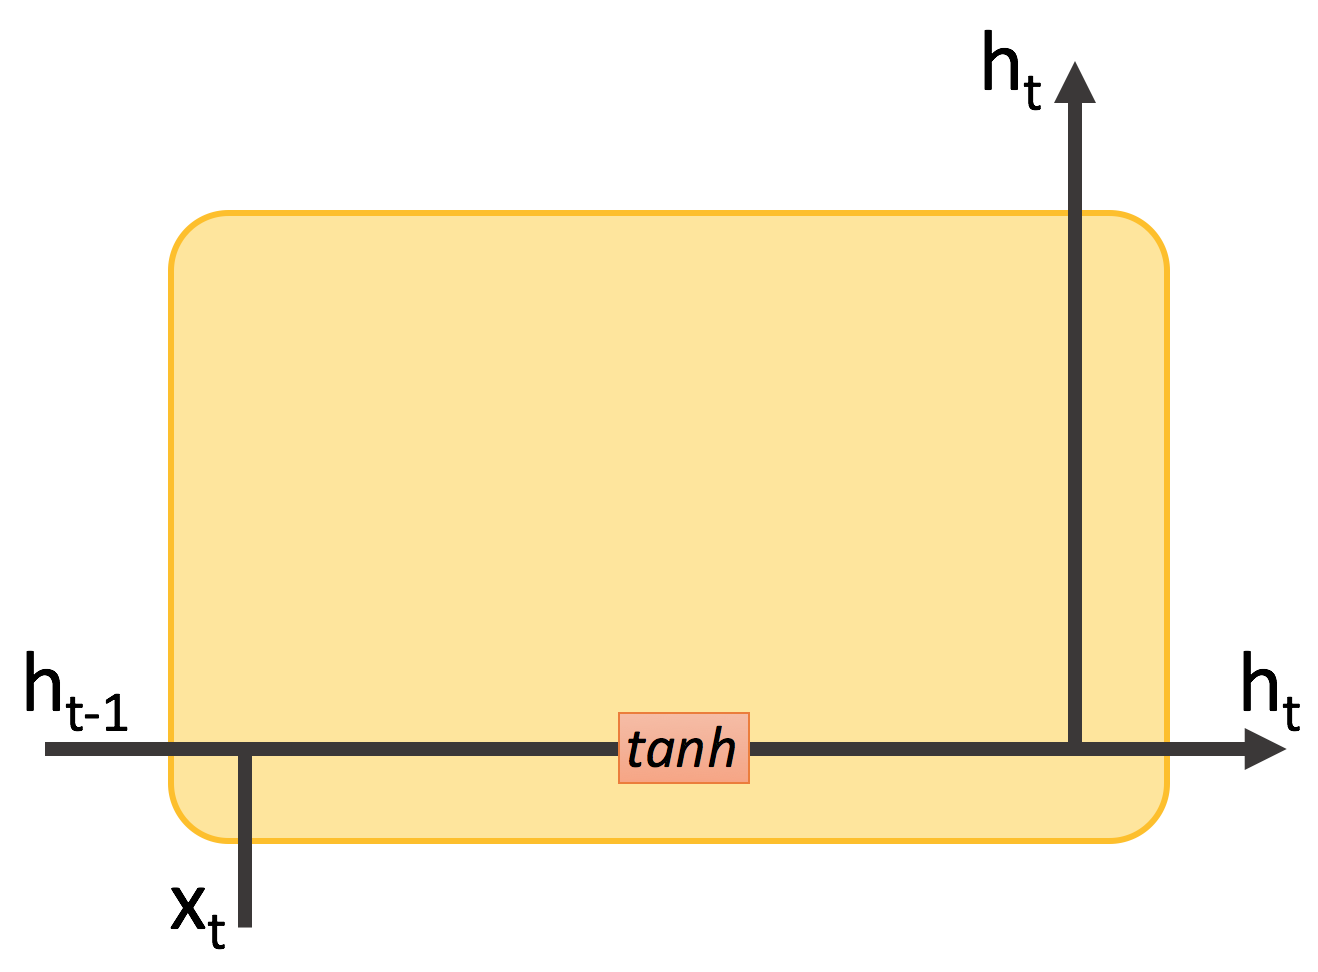
\includegraphics[scale=0.3]{images/chap2_rnnstruct.png}
    \caption{遞迴式網路架構}\label{fig:chap2_rnnA}
\end{figure}
我們由左至右來看。首先,先決定哪些資訊需要從單元狀態中拋棄,通過一個遺忘閘 $f_t$(Forget Gate)來處理。它接收了現在這個時間點的資訊以及上個時間點的隱藏狀態(Hidden State),分別通過一層線性矩陣轉換投影到同一個維度並相加,再通過一個 S 型函數,成為一個 0 到 1 所組成的向量,參考式子(\ref{function:forget})及圖 \ref{fig:forget} ,跟 $C_{t-1}$ 來進行逐點乘積(Pointwise Product),因此若 $f_t$ 值為 0 代表要清除之前儲存的內容,而 1 代表完全保留。
\begin{figure}[h]
    \centering
    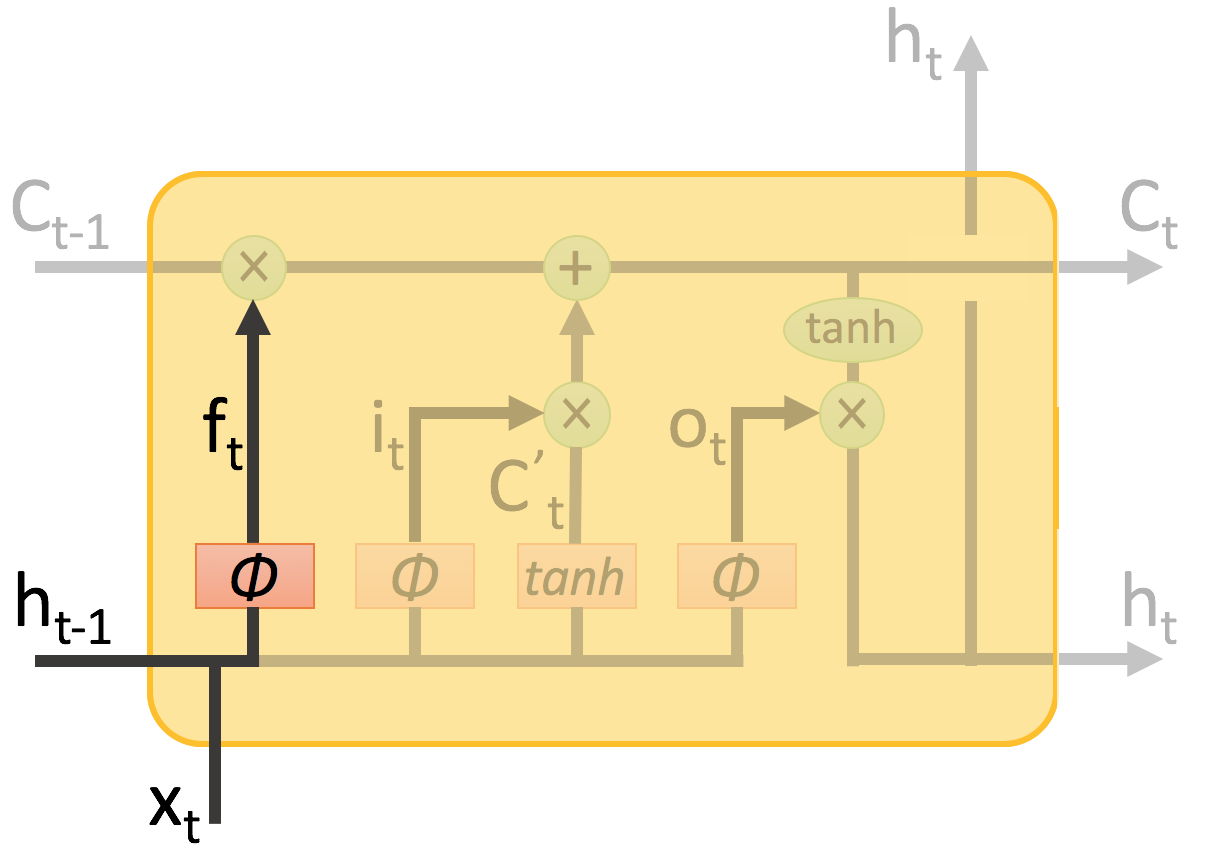
\includegraphics[scale=0.35]{images/chap2_forget.png}
    \caption{遺忘閘示意圖\cite{shen2016} }\label{fig:forget}
\end{figure}
\begin{equation}
    f_t = \phi(W_{xf}x_t + W_{hf}h_{t-1} + b_f) \label{function:forget}
\end{equation}

再者,我們需要決定哪些要被儲存進管理單元中,稱為輸入閘(Input Gate)$i_t$ ,為 S 型函數決定要更新多少資訊,類似遺忘閘 $f_t$ 的概念,如式子(\ref{function:input_gate})。而至於要更新至管理單元的資訊,則是由另一個非線性函數雙曲正切(Hyperbolic Tangent, Tanh)負責產生出候選值 $C_t^{'}$ ,參考式子(\ref{function:candidate})及圖 \ref{fig:input_gate}。
\begin{figure}[h]
    \centering
    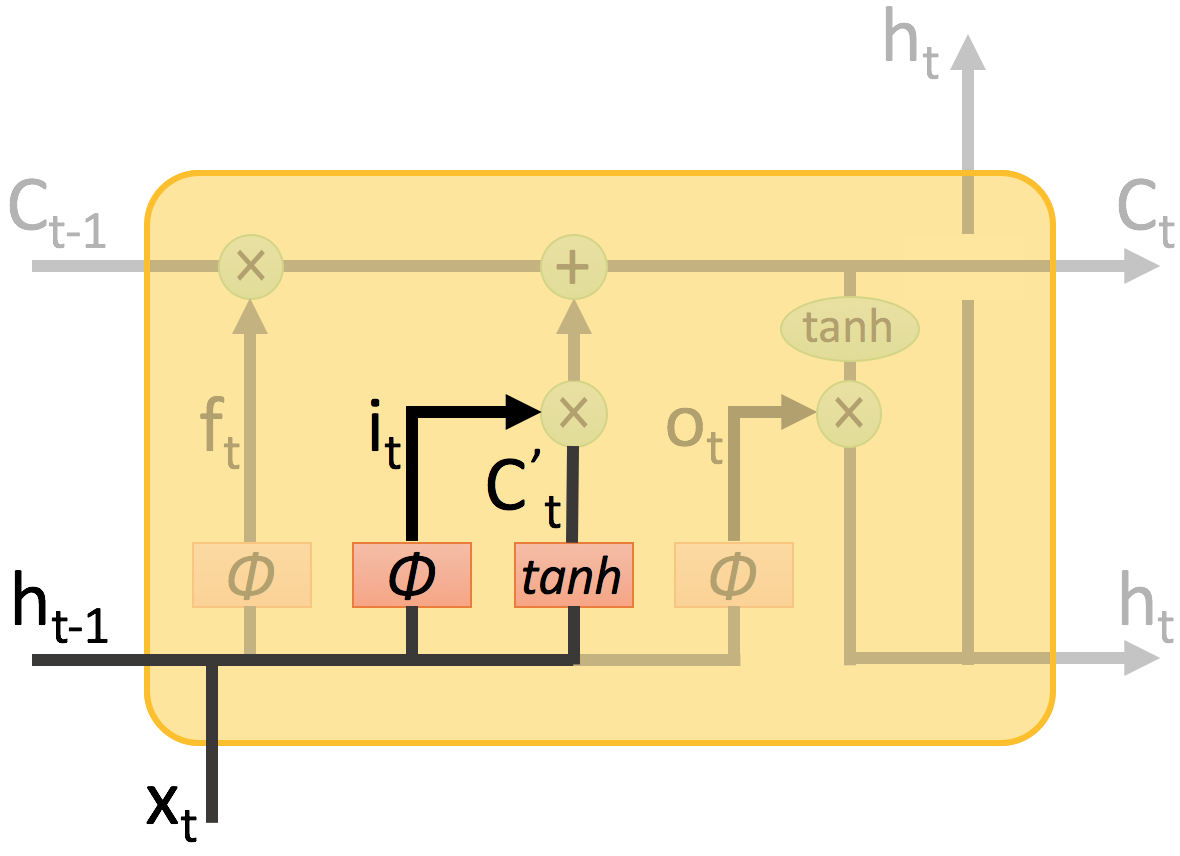
\includegraphics[scale=0.35]{images/chap2_input.png}
    \caption{輸入閘示意圖\cite{shen2016} }\label{fig:input_gate}
\end{figure}
\begin{equation}
    i_t = \phi(W_{xi}x_t + W_{hi}h_{t-1} + b_i) \label{function:input_gate}
\end{equation}
\begin{equation}
    C_t^{'} = tanh(W_{xC}x_t + W_{hC}h_{t-1} + b_C) \label{function:candidate}
\end{equation}
更新管理單元的方法,只需要將上一個管理單元 $C_{t-1}$ 搭配由雙曲正切產生出的候選值 $C_t^{'}$ ,分別根據 $f_t$ 與 $i_t$ 進行加權和,如此便能更新單元狀態 $C_t$ ,如式子(\ref{function:update})及圖 \ref{fig:update}。
\begin{figure}[h]
    \centering
    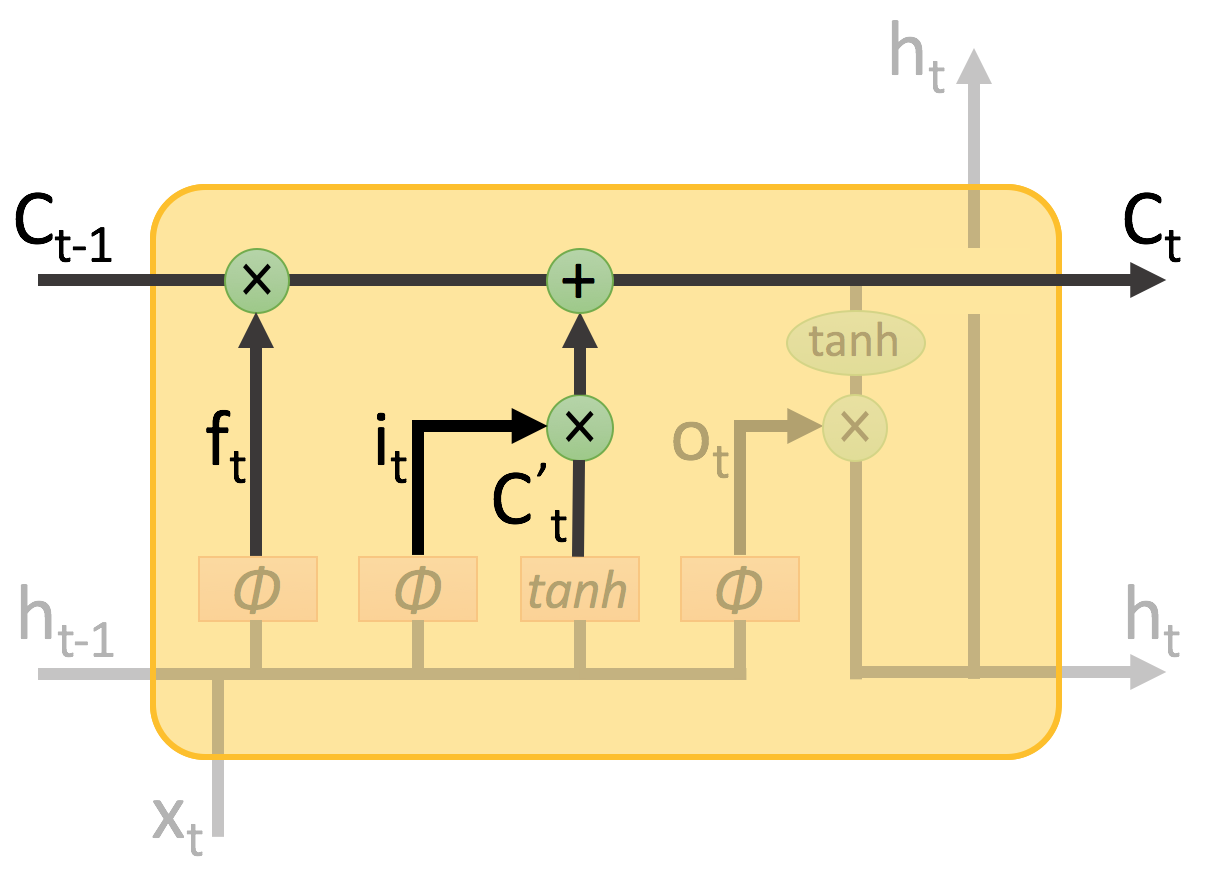
\includegraphics[scale=0.35]{images/chap2_update.png}
    \caption{更新管理單元狀態\cite{shen2016} }\label{fig:update}
\end{figure}
\begin{equation}
    C_t = f_t * C_{t-1} + i_t * C_t^{'} \label{function:update}
\end{equation}
最後一個則是輸出閘(Output Gate)$o_t$ ,跟前兩個門閘一樣,控制多少比例要輸出,如式子(\ref{function:output})。接著管理單元通過雙曲正切函數,使得輸出值介於 -1 到 1 之間,與輸出閘逐點乘積,這樣便可以只更新想要的隱藏狀態,如式子(\ref{function:hidden_state})及圖 \ref{fig:output_gate}。
\begin{figure}[h]
    \centering
    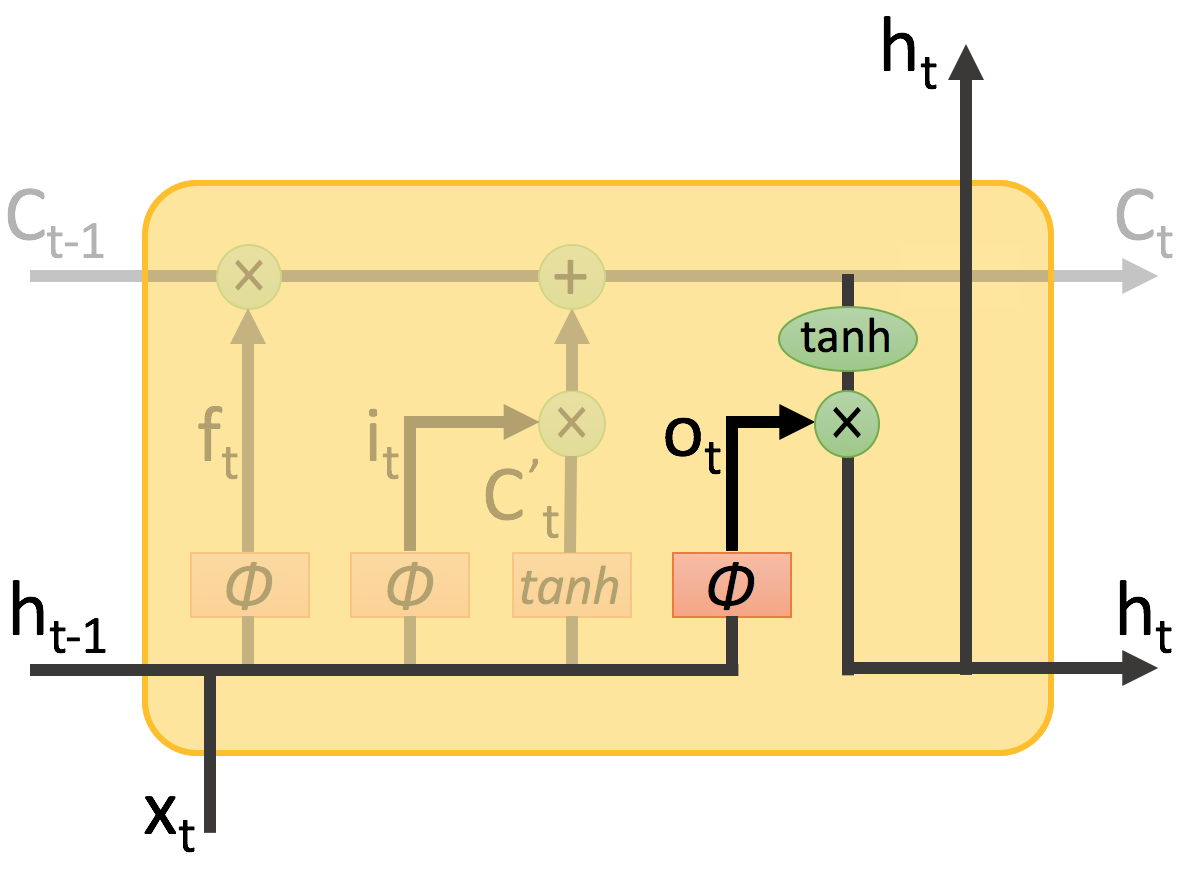
\includegraphics[scale=0.35]{images/chap2_output.png}
    \caption{輸出閘示意圖\cite{shen2016} }\label{fig:output_gate}
\end{figure}
\begin{equation}
    o_t =  \phi(W_{xo}x_t + W_{ho}h_{t-1} + b_o) \label{function:output}
\end{equation}
\begin{equation}
    h_t = o_t * tanh(C_t) \label{function:hidden_state}
\end{equation}

由式子(\ref{function:forget})到(\ref{function:output})可明顯看出,門閘的權值都是由 $x_t$ 和 $h_{t-1}$ 所計算而成,但由三組參數組合而成,容易造成過度貼合。因此之後有人提出了長短期記憶網路的簡化版,是門閘遞迴單元(Gated Recurrent Unit, GRU)~\cite{cho2014learning} ,將輸入閘和遺忘閘組合為更新閘(Update Gate)$z_t$ ,其精神是「舊的不去,新的不來」,也合併了管理單元與隱藏狀態,如式子 \ref{function:gru} 及圖 \ref{fig:gru}。相較於長短期記憶網路而言,使用的參數量也較少,模型更簡單一些,也因此較為流行,本碩論也採用門閘遞迴單元。
\begin{figure}[h]
    \centering
    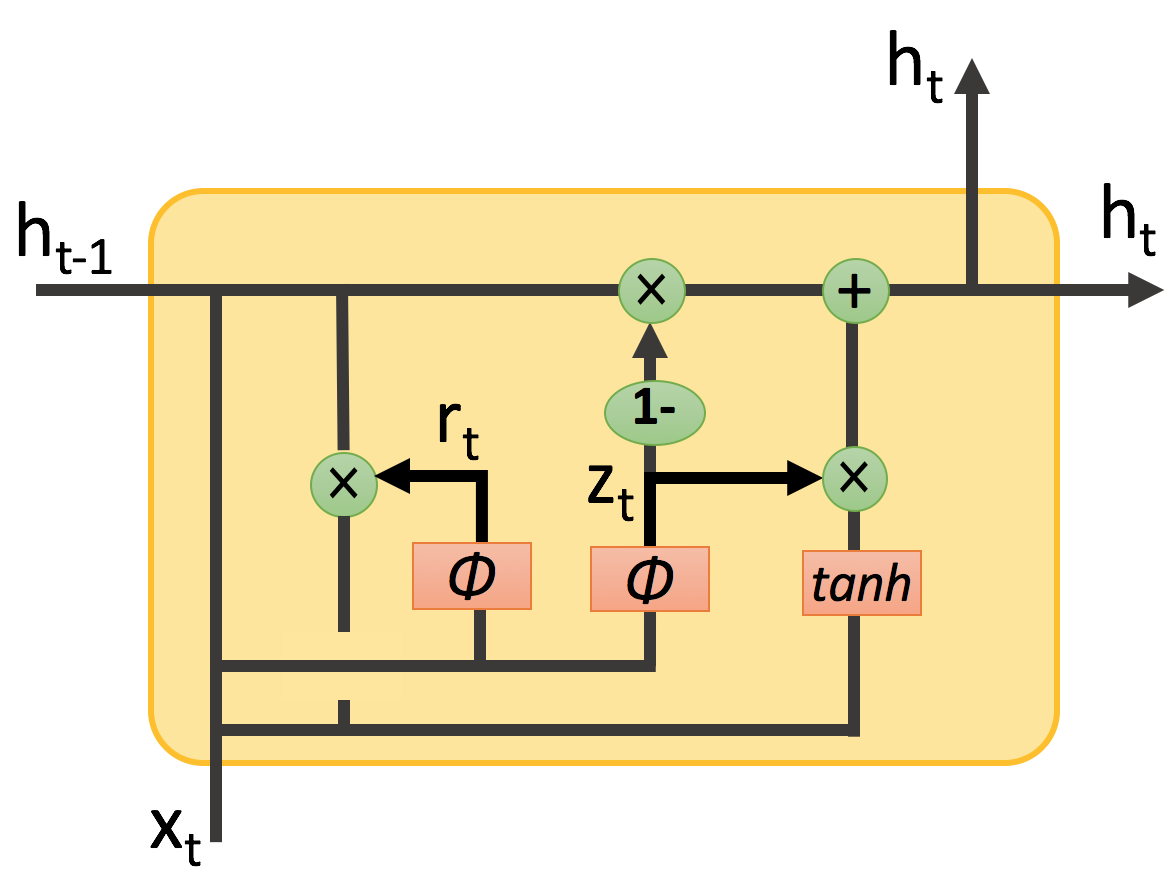
\includegraphics[scale=0.35]{images/chap2_gru.png}
    \caption{門閘遞迴單元}\label{fig:gru}
\end{figure}
\begin{equation}
    \label{function:gru}
    \begin{aligned}
        z_t = \phi(W_z [h_{t-1},x_t]) \\
        r_t = \phi(W_r [h_{t-1},x_t]) \\
        \tilde{h_t} = tanh(W[r_t*h_{t-1},x_t]) \\
        h_t = (1-z_t) * h_{t-1} + z_t * \tilde{h_t}
\end{aligned}
\end{equation}
\subsection{序列對序列模型}
遞迴式神經網路使得深層類神經網路突破了傳統固定大小輸入的框架,而序列對序列模型(Sequence to Sequence Model)首先用於翻譯這一類型的序列式問題,並且在英語-法語翻譯應用中有著良好的表現。

首先由班氏(Bengio)提出編碼器-解碼器(Encoder-Decoder)的架構\cite{cho2014learning},為序列對序列模型的雛形,而 Google Brain 的蘇氏(Sutskever)則是完整定義出序列對序列模型的概念 \cite{sutskever2014sequence} 。

編碼器-解碼器模型的核心思想是通過長短期記憶神經網路,將一段輸入的序列映射結果,作為一個輸出的序列,而這一個過程可分為編碼輸入以及解碼輸出兩個環節所組成。如圖 \ref{fig:seq2seq} 所示,在這個模型中每一時間點的輸入與輸出是不一樣的。比如說我們現在有序列 A、B、C、$\langle$ EOS $\rangle$($\langle$ EOS $\rangle$ 為 End-of-Sentence,代表句子結尾。)作為輸入,那們我們的目的就是將 A、B、C、$\langle$ EOS $\rangle$ 依序傳入模型後,再映射出序列 X、Y、Z、$\langle$ EOS $\rangle$ 作為輸出。

\begin{figure}[h]
    \centering
    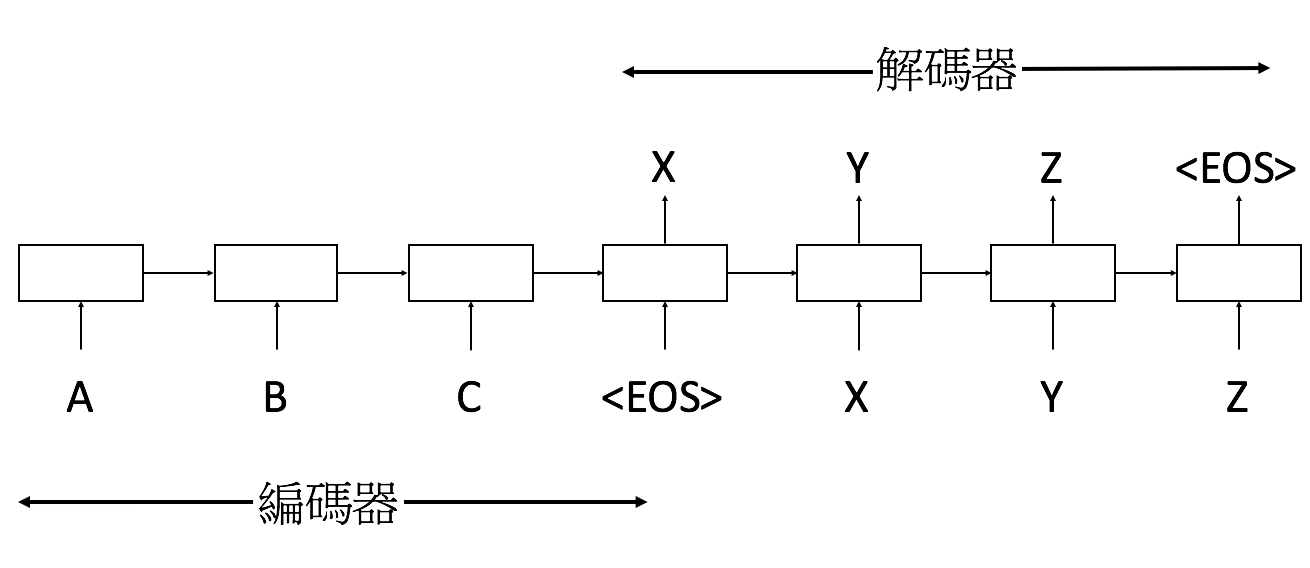
\includegraphics[scale=0.5]{images/chap2_seq2seq.png}
    \caption{序列對序列模型}\label{fig:seq2seq}
\end{figure}

序列對序列模型的目標是為了模擬此條件機率 $p(y_1,...,y_{T'}|x_1,...x_T)$ ,並使其值最大化,而此條件機率可表示為式子 \ref{function:cond} 。此模型可以拆成兩個部分解讀,前者為編碼器,而後者為解碼器。
\begin{equation}
    p(y_1,...,y_{T'}|x_1,...x_T) = \prod_{t=1}^{T'}p(y_t|y_1,...y_{t-1},c) \label{function:cond}
\end{equation}

第一部分是把不定長度(Variable-length)的輸入序列 $(x_1,...,x_T)$ 經由遞迴式神經網路所建構的編碼器編譯為上下文向量 $c$(Context Vector),如式子 \ref{function:encoder} ,通常會取最後一個隱藏狀態 $h_T$ ,或者是所有 $h_1,...,h_t$ 的加權總和做為一固定長度的向量表示(Fixed-lnegth Vector Representation)。
\begin{equation}
    h_t = f(x_t, h_{t-1});\quad  c = \phi(\{h_1,...,h_T\}) \label{function:encoder}
\end{equation}

編碼完以後,第二部分則是根據這個固定的長度向量再通過一個遞迴式類神經網路解碼器裡進行解譯,如式子 \ref{function:decoder} ,用來產生(Generate)輸出序列,通常會使用貪婪(Greedy)演算法,在每個時間點 $t$ 時選出最大機率的 $y_t$ ,或者是透過集束搜尋(Beam Search),選出滿足式子 \ref{function:cond} 的最大機率作為輸出序列。

\begin{equation}
    h_t = f(h_{t-1},y_{t-1},c); \quad p(y_t|y_{<t},X) = g(y_{t-1},s_t,c) \label{function:decoder}
\end{equation}

遞迴式神經網路有許多種類的應用,如一對多的字幕生成器(Caption Generation),透過一張圖片,產生適合的文字;或多對一的如情感分析(Sentiment Analysis),來分析一段句子潛在的情感;或者是多對多的如機器翻譯(Machine Translation)等等廣泛的被使用在各個自然語言領域。

\section{詞彙表示法 - 詞嵌入(Word Embedding)}
\subsection{基本介紹}
深層學習近年來在自然語言處理領域中已經開拓出越來越大的新空間,而詞嵌入(Word Embedding)可說是其中具有相當重要意義的一項工具。傳統上,為了將一個自然語言中所有的詞以數學符號形式呈現,並進行各式自然語言處理問題,最常使用的表達方式是 1-of-N 編碼(1-of-N Encoding),意思是每個詞都被表示成一個維度 $N$ 的詞向量(Word Vector), $N$ 為整個詞典的大小,且詞典中的每個詞都對應到一個特定的維度,而一個詞向量只有在該詞所對應到的維度其值為 1 ,其他 $N-1$ 個維度的值都是 0 ,這種表示方式雖然非常的稀疏(Sparse),但其意義卻相當簡潔明瞭, 1 所在的維度即說明了這個詞向量是辭典中的哪個詞,且事實上 1-of-N 編碼在許多問題上,搭配許多機器學習模型進行訓練後都有不錯的表現。

然而 1-of-N 編碼有幾個缺點。首先,由於自然語言辭典 $N$ 的大小一般來說都在數萬至數十萬的量級,因此這種詞向量的維度也非常大,在機器學問題上很容易受到維度災難(Curse of Dimensionality)之影響,使表現變差。再者,這種表現方式將詞典中任意兩個詞都視為獨立,完全無法呈現出兩個詞之間的語意關係,就算是兩個同義詞(Synonym),或是詞性變換,他們的 1-of-N 編碼之間也毫無關聯。因此在 1986 年,分佈式表達(Distributed Representation)的概念首次被提出,以分佈式表達呈現出的詞向量不僅維度遠低於辭典大小 $N$ ,且每個維度上的值可以是任意的連續實數,所以透過計算兩個向量之間的歐式距離或是餘弦相似度(Cosine Similarity)之大小,兩者之間的語意關係就能呈現出來,而這些向量所在之空間即稱為語意空間(Semantic Space)。此技術產生之詞向量我們將之稱為分佈式詞彙表達法(Distributed Word Representation),或者稱為詞嵌入。
%(Euclidean distance)

詞嵌入在諸多自然語言處理問題上已經被證明相當有幫助,例如專有名詞辨識(Name Entity Recognition)、詞性標註、句法分析(Syntactic Parsing)、語意分析(Semantic Analysis)、情感分析(Sentiment Analysis)、機器翻譯等等。詞嵌入的訓練與抽取方式並不唯一,過去已有眾多方法被研究提出,一種是訓練語言模型(Language Model)時所得到的副產物,另一種則是使用特別設計的模型,模擬每個詞與其上下文(Context)之間的關係。%由於本論文之研究並未使用前者技術,因此在接下來的段落只會對後者進行詳細介紹。
\subsection{跳躍文法模型(Skip-gram Model)}
跳躍文法模型(Skip-gram Model)是由米式於 2013 年提出 ~\cite{mikolov2013distributed}~\cite{mikolov2013efficient} ,是一個利用類神經網路來訓練的模型,如圖 \ref{fig:skip_gram} 所示,跳躍文法模型可以分為三個層級:
%(Tomas Mikolov)
\begin{figure}[h]
    \centering
    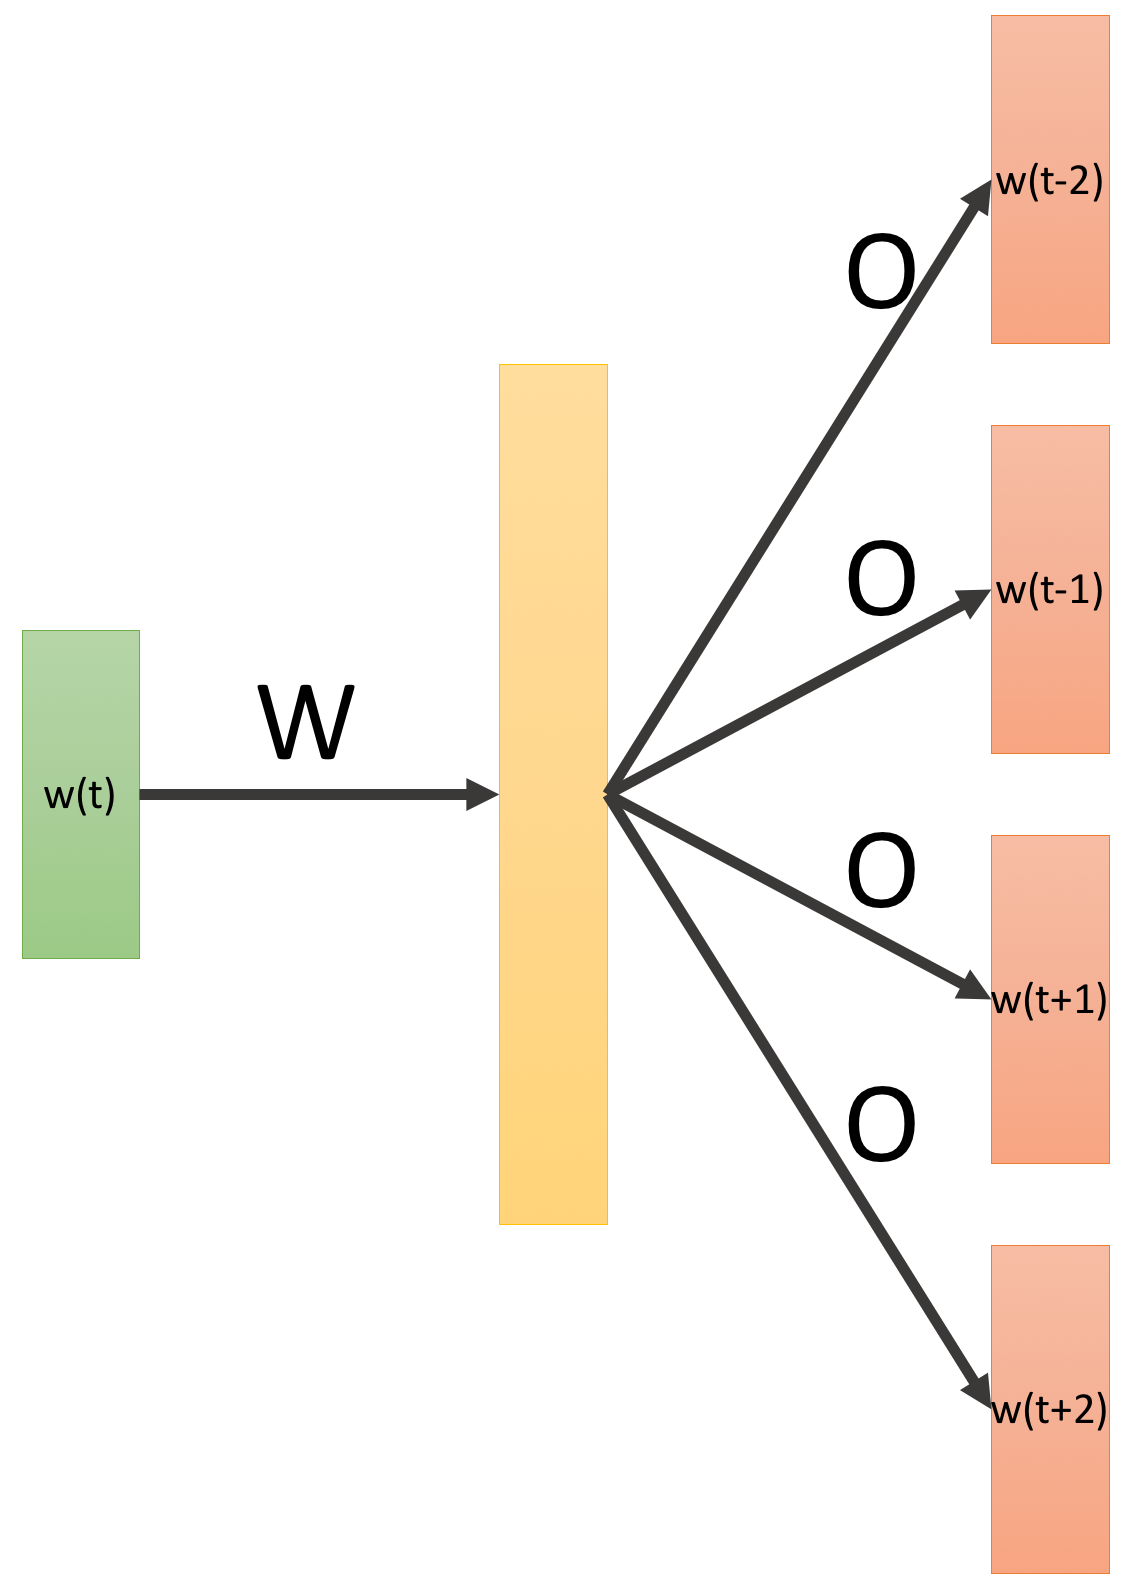
\includegraphics[scale=0.35]{images/chap2_skipgram.png}
    \caption{跳躍文法模型示意圖 \cite{shen2016} }\label{fig:skip_gram}
\end{figure}
\begin{itemize}
    \item 輸入層:是一個與辭典大小同長度的陣列,採用 1-of-N 編碼形式,而只有該索引的位置之值為 1 ,其餘皆為 0 。此向量用來表示當前詞 $w(t)$ 作為輸入。
    \item 輸出層:每一個矩形都是與辭典大小同長度的陣列,也採用 1-of-N 編碼形式,而只有某一維度的值為 1 ,其餘皆為 0 。不過每一個矩形是代表前後文的詞,例如 $w(t-2)$、$w(t-1)$、$w(t+1)$、$w(t+2)$ ,我們希望透過跳躍文法模型來預測出當前詞的上下文機率分佈。
    \item 隱藏層:通常維度較小,同時也是代表詞向量的維度。代表的是該時間點當前詞 $w(t)$ 透過隱藏層與輸入層之間的一組權重矩陣 $W$ 投影後的向量。和一般類神經網路的隱藏層不同,此投影後的向量不會再通過任何非線性的函數,而投影到 $w(t-2)$、$w(t-1)$、$w(t+1)$、$w(t+2)$ 等所有輸出層之間,都存在一組共享的權重矩陣 $O$ ,把 $w(t)$ 投影後的向量再做一次線性轉換,預測當前這個詞的上下文機率分佈。
\end{itemize}

跳躍文法模型是專為詞嵌入的抽取而設計的模型,而其抽出之詞嵌入即為權重矩陣 $W$ 中的每一行%(Column)
,或換個說法,是 $w(t)$ 經過 $W$ 的投影結果。此模型同樣也是利用反向傳播演算法進行訓練。通常當預測的上下文範圍越大,得到的詞嵌入品質越好,但同時也大幅增加了計算上的複雜度,而且一般來說和當前詞距離越遠的上下文,和當前詞的相關性越低,所以在訓練時,距離越遠的上下文取樣次數會越少,以降低它的影響力。舉例來說,若設定最大上下文的範圍是 $C=5$ ,每次訓練時都會隨機選擇一個數字 $R$ 介於 1 到 C 之間,並且以當前詞過去的 $R$ 個詞至未來 $R$ 個詞,總共 $2R$ 個詞作為模型輸出層要預測的目標。

\section{機器閱讀理解數據集(MAchine Reading COmprehension, MARCO, Dataset)}
\subsection{問答系統}
問答系統可以視為資訊檢索之延伸,在資訊檢索的情形下,系統針對使用者所輸入的查詢詞(Query)回傳相關的文本,然而隨著科技的發展與資訊量的爆炸,我們不只要系統提供給我們文本,甚至是能夠直接提供查詢詞所對應的答案,如此一來,在面對龐大的資料量時,我們便能快速找出符合查詢詞,直接將可能的答案回傳,以方便使用者閱覽。

問答系統可根據問題類型來分成幾類,最基本的是仿真陳述問答(Factoid Question Answering),此類系統是根據所提供資訊,答案的正確與否是根據所提供的內容來決定,在現實生活中不一定為真,故稱為仿真陳述問答。若是要求簡述某個定義,如「語音文件的定義為何?」,則稱為定義式問答(Definitional Question Answering),通常文字描述會不太一樣,但語義應該是一致的。另外有一種是要求問答系統如「請列舉台灣有哪些縣市?」,此種稱為清單問答(List Question Answering)。除了這些與問句資訊有關的類型外,最近評鑑會議引進如「時間限制問題」(Temporally Restricted Question)之複雜的問題類型,時間限制型的問題會在問句中明確指出答案的時間範圍限制,比如說以「民國一百年時的台灣總統是誰?」這問句來說,系統必須有根據答案語料結構化資料,或上下文來推論正確答案的能力。而過去常見處理這類型的問題,通常會將文本的每個句子與查詢詞解析(Parse)成三元組(Triplet),並試圖從所有三元組中,找出所有符合查詢詞所解析之三元組。

在深度學習中,大量的數據是必備的,才能夠有效且成功地訓練出好的模型,也因此各個領域紛紛釋出大量的數據集,已讓多個領域有著顯著的突破,如在圖像領域中,有大規模圖像識別競賽(Large Scale Visual Recognition Challenge, ILSVRC)釋出的 ImageNet \cite{imagenet_cvpr09} ,其中包含 150 萬張圖片與其圖片所包含物件的種類共 1000 個;在語音領域中,則有 TIMIT 、 Switchboard 、 LibriSpeech 等高達 1000 小時的語音語料(Corpus),然而,在閱讀理解(Reading Comprehension, RC)相對於其他領域的語料庫而言,並沒有如此大量的語料,抑或是各有著顯著的缺點,如:數據集可能不夠大量、文章是機器合成的(Synthetic)等等。
%問答系統和資訊檢索(Information Retrieval)系統最大的不同在於,問答系統只針對使用者輸入的問句回傳對應之答案,而不是提供使用者先關的資訊,讓使用者自己找答案。此種系統的優點是,面對龐大的資料量或者是很多複雜內容的文本時,使用者有時候無法從眾多文字中找出對應的答案,因此問答系統透過文字處理,直接將可能的答案回傳,以方便使用者閱覽。

%通常問答系統可以根據答案種類分成三種,仿真陳述問答(Factoid Question Answering)、定義式問答(Definitional Question Answering)、以及複雜式問答(Complex Question Answering)。最基本的類型為仿真陳述問答,此系統根據答案與料所述資訊,取出一小段字串作為答案,由於答案的正確與否是根據答案語料的內容來決定,在現實生活中不一定為真,故稱為仿真陳述問答。而定義式問答通常是要求簡述某個定義,其回答因為自然語言的表達方法有很多,通常答案不會一致,但語義應該是相近的,複雜式問答系統通常沒有一個標準答案,往往跟回答者的主觀想法或者立場有關,因此被視為最困難且難以評估的一種問答,諸如「台灣大學附近的推薦美食有哪些?」。除了這些與問句資訊有關的類型外,最近評鑑會議引進如「時間限制問題」(Temporally Restricted Questions)與「序列問題」(Series of Questions)等複雜的問題類型。時間限制型的問題會在問句中明確指出答案的時間範圍限制,比如說以「民國一百年時的台灣總統是誰」這問句來說,系統必須有根據答案語料結構化資料,或上下文來推論正確答案的能力。
%\subsection{}
%\subsection{知識為基礎之問答系統}
%
%\subsection{類神經網路之問答系統}
\subsection{語料介紹}
過去幾個著名的閱讀理解的數據集有如 Facebook 的 bAbi \cite{weston2015towards}  、 Microsoft 提供的 MCTest \cite{richardson2013mctest} 和 WikiQA \cite{yang2015wikiqa} 、 Google 所彙集 CNN 和每日郵報 \cite{hermann2015teaching} 的新聞以及史丹佛(Stanford)收集在維基百科相關的約莫 100,000 個問答對(Question-Answer Pair)和 500 多篇文章的數據集,稱為 The Stanford Question Answering Dataset ,簡稱 SQuAD \cite{rajpurkar2016squad} 。然而上述語料各有其致命缺點,舉例來說,bAbi 的句子皆是機器生成的,整體的詞彙大小(Vocabulary Size)非常小,且答案只會是一個單一詞彙,如圖 \ref{fig:babi} 、 MCTest 是多重選擇題,而真實世界中並不可能有選項讓機器回答、 WikiQA 則是只有約莫 2K 的問答句子,並不夠讓我們訓練出夠深的模型、SQuAD 雖然有十萬左右的問答對,但其答案必定是在文章的某個段落,在真實世界的問答中,答案不可能皆是文章的某個段落。

\begin{figure}[h]
    %\centering
    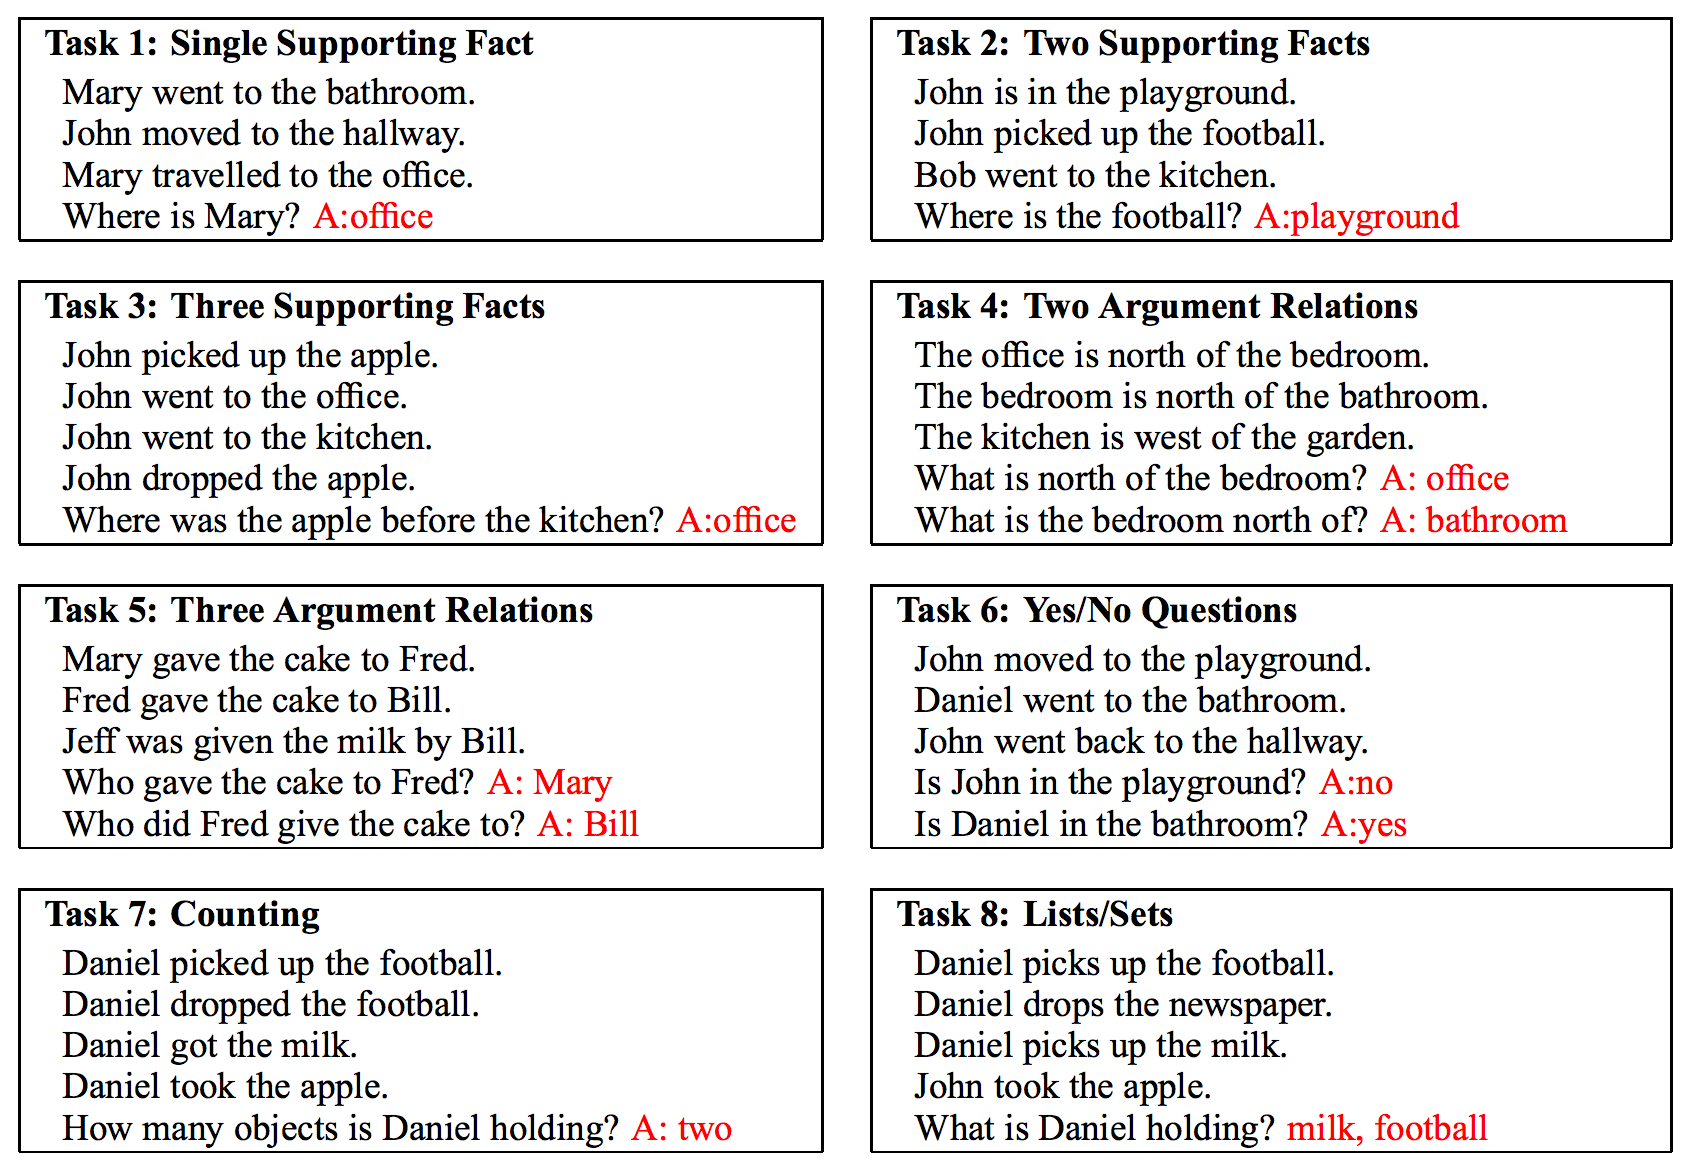
\includegraphics[scale=0.6]{images/chap2_babi.png}
    \caption{Facebook bAbi 範例}\label{fig:babi}
\end{figure}

%,數據集的相關介紹如表 \ref{table:dataset} 
為了促進閱讀理解的發展, Microsoft 因此釋出了機器閱讀理解數據集(MAchine Reading COmprehension, MARCO, Dataset)\cite{nguyen2016ms} ,此數據集是由微軟根據使用者在 Bing 搜尋結果所得之文本,並由人們眾包(Crowdsourcing)所得到的答案。跟其他數據集相比,資料量夠大、不是人工生成的數據(Artificially Generated Data)、答案亦是由人們所產生。表(\ref{table:dataset})是閱讀理解數據集之比較。

\begin{table}
    \caption{數據集介紹}
    \label{table:dataset}
    \centering
    \begin{tabular}[t]{|l|l|l|l|}
        \hline 
        數據集          &回答問題方式   &問題數目   &文章數目 \\
        \hline
        bAbi            &單一詞彙       &約10K      &  \\
        \hline
        MCTest          &多重選擇題     &2640       &660 \\
        \hline
        WikiQA          &句子選擇       &3047       &29.26K\\
        \hline
        CNN/每日郵報    &克漏字填空     &1.4M       &93K CNN,220k DM\\
        \hline
        SQuAD           &文章區間       &100K       &536\\
        \hline
        MS MARCO        &人類生成       &100K       &200K+文章\\
        \hline
    \end{tabular}
\end{table}
%\begin{table}
%    \caption{問句包含詞比例}
%    \label{table:query_percentage}
%    \centering
%    \begin{tabular}[t]{|l|l|}
%        \hline
%        問句包含    &比例\\
%        \hline
%        what        &42.2\%\\
%        \hline
%        how         &15.3\%\\
%        \hline
%        where       &4.4\%\\
%        \hline
%        when        &2.0\%\\
%        \hline
%        why         &1.8\%\\
%        \hline
%        who         &1.7\%\\
%        \hline
%        which       &1.4\%\\
%        \hline
%    \end{tabular}
%\end{table}
%\begin{table}
%    \caption{答案種類}
%    \label{table:query_type}
%    \centering
%    \begin{tabular}[t]{|l|l|}
%        \hline
%        描述(Description) &52.6\%\\
%        \hline
%        數字(Numberic)    &28.4\%\\
%        \hline
%        名詞(Entity)      &10.5\%\\
%        \hline
%        地點(Location)    &5.7\%\\
%        \hline
%        人物(Person)      &2.7\%\\
%        \hline
%    \end{tabular}
%\end{table}
